\section{Methodology} \label{methodology}

Lorem ipsum dolor sit amet, consectetur adipiscing elit. Pellentesque auctor nec turpis eget placerat. Integer ac massa cursus, porttitor libero et, tincidunt lectus. Morbi pulvinar at leo vitae rutrum. Proin congue facilisis ex et laoreet. Nulla id metus pulvinar sem scelerisque convallis. Aliquam varius urna ut massa euismod varius. Etiam volutpat, urna et convallis eleifend, tellus risus tincidunt leo, porttitor sagittis eros felis ut nisi. Suspendisse semper mi quam, vitae mattis dolor volutpat non. Nam lacinia posuere est, at aliquam nulla consequat vel. Etiam suscipit, sem a tempus condimentum, sapien arcu luctus est, et consequat nunc diam id nulla.

\begin{figure} [h]
\centering
\def\svgwidth{0.6\columnwidth}
\input{Figures/Chap-3/pie-chart-text.pdf_tex}
\caption{Inkscape graph with 'pdf\_tex'}
\label{fig:graph-inkscape-tex}
\end{figure}

Donec ut erat massa. Vivamus vel lobortis magna. Sed varius, sem vel facilisis tempus, dui magna tempus nisl, et maximus libero leo at lorem. Vestibulum ante ipsum primis in faucibus orci luctus et ultrices posuere cubilia Curae; Proin laoreet nulla dolor, sit amet consectetur risus finibus in. Vestibulum nec euismod nisl, a pretium urna. Sed interdum purus sed dapibus facilisis. Cras consectetur tempus dui, eu tempor dui aliquet vitae. Integer bibendum pellentesque felis, volutpat iaculis mi sagittis ac. Fusce vel eros purus. Pellentesque pulvinar libero quis nisl pharetra, ut mattis turpis efficitur. Phasellus dui nisi, rhoncus ac nunc quis, pulvinar lobortis massa. Vestibulum ac libero lectus. Nunc nec malesuada diam. Cras rutrum, velit sed mattis efficitur, leo turpis faucibus ligula, a tristique ligula massa sit amet massa, as shown in Figure \ref{fig:graph-inkscape-tex} (created with Inkscape and exported as PDF+LaTeX).

\begin{figure}[htp]
\centering
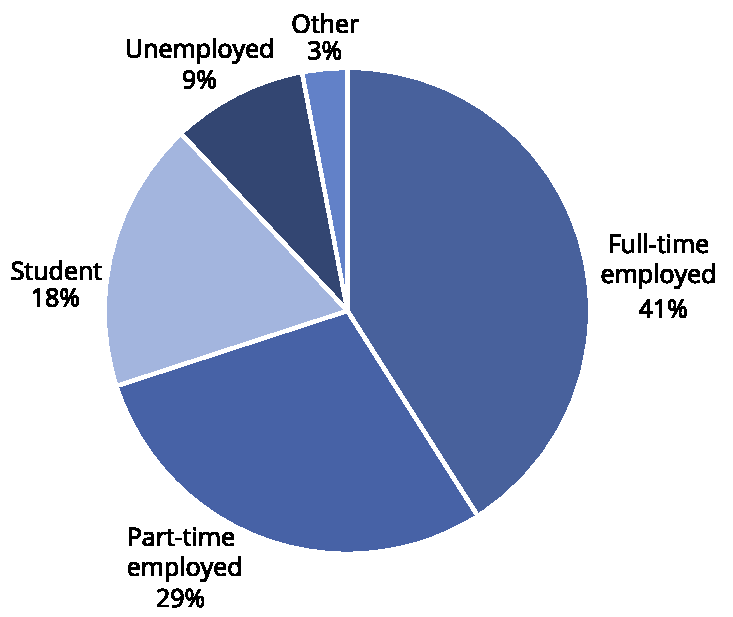
\includegraphics[width=7cm]{Figures/Chap-3/pie-chart.pdf}
\caption{Regular Inkscape graph}
\label{fig:graph-inkscape}
\end{figure}

Morbi egestas felis ipsum, nec fermentum massa pharetra vel. Proin congue pulvinar urna vitae pharetra. Nunc elementum dignissim vehicula. Ut ac iaculis nibh, ac aliquam ipsum. Fusce quis tincidunt nisi. Maecenas rhoncus sapien et ipsum elementum maximus. Interdum et malesuada fames ac ante ipsum primis in faucibus. Aenean ultrices erat justo, id eleifend libero lacinia eget. Aenean feugiat finibus interdum. In consequat lobortis enim in volutpat. Nullam egestas sed erat ut tempor. Cras ut libero ligula. Donec cursus imperdiet sagittis. Nam id tempor erat. Suspendisse molestie vel nisi sit amet hendrerit, as shown in Figure \ref{fig:graph-inkscape} (created with Inkscape, and exported as a regular PDF).


\begin{center}
\captionof{diag}{Test with smartdiagram}
\smartdiagram[bubble diagram]{Energy Technologies,
  Solar-PV, Wind, Hydro, Tidal, Biomass}
\end{center}

Donec eu cursus sapien. Sed ornare, nulla ac dapibus mollis, augue dui tempor odio, eget dictum dolor tortor vitae ipsum. Donec scelerisque justo rutrum tellus pellentesque euismod. Integer aliquet neque id ante tincidunt rhoncus. Cras blandit purus sit amet condimentum rhoncus. In scelerisque mauris eget quam sollicitudin accumsan. Nulla lobortis dapibus magna, eget blandit arcu ullamcorper et. Donec porta ullamcorper lectus ut feugiat. Sed diam dolor, molestie quis hendrerit vel, semper sed lectus. Ut ac enim enim. Donec fringilla nunc ipsum, quis aliquam leo consequat ac. Class aptent taciti sociosqu ad litora torquent per conubia nostra, per inceptos himenaeos-

\begin{figure}[h]
\centering
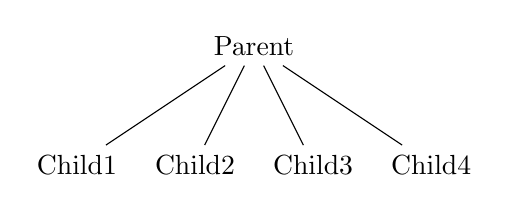
\begin{tikzpicture}
\node{Parent}
	child { node {Child1}}
	child { node {Child2}}
	child { node {Child3}}
	child { node {Child4}}
;
\end{tikzpicture}
\caption{Figure made with TikZ} \label{fig:tikz}
\end{figure}

Etiam condimentum tincidunt nibh eget facilisis. Pellentesque vel est efficitur, viverra purus mattis, mattis purus. Cras ac mattis nulla. Sed pulvinar sollicitudin nunc, in auctor libero iaculis non. Ut eu sem quis risus ultrices elementum in quis enim. Suspendisse cursus, mi eget posuere vulputate, magna erat maximus justo, sit amet imperdiet metus purus at dui. Nunc pulvinar augue mattis dui tristique, eu iaculis neque maximus. Donec porta imperdiet rhoncus. Morbi vitae mauris elementum, semper quam condimentum, rhoncus eros. Mauris metus felis, hendrerit nec imperdiet id, vestibulum eu felis. Sed aliquam euismod ex, sed cursus ante molestie nec, as shown in \ref{fig:tikz} (made with TikZ).